\chapter{State of the Art}
\label{ch:state-of-the-art}

\section{The DNS System: Background}
\label{subsec:2.1}

The \ac{DNS} is the distributed directory that translates human-readable names into machine-readable information — primarily \ac{IP} addresses~\cite{RFC1034,RFC1035}. Its hierarchy mirrors the delegation of administrative authority: the root zone delegates to \ac{TLD}s, which delegate to authoritative name servers for individual domains. Resolution is performed by a recursive resolver acting on behalf of clients — contacting root, \ac{TLD}, and authoritative servers in sequence and caching results for the duration of each record's \ac{TTL}.

Every \ac{DNS} record carries a \ac{TTL}. \ac{CDN} A records are typically 60 seconds — sometimes 30. NS and SOA records at the same domain may be valid for 86\,400 seconds. That spread matters for measurement. A recursive resolver may serve an answer cached several minutes ago. Two probes returning different \ac{IP}s could be observing geographic routing, or simply different cache states from staggered refresh times. There is no way to tell which, from the recursive side. Querying the authoritative server directly cuts out the cache layer.

\subsection{Resource Record Types Relevant to Measurement Studies}
\label{sec:2.1.1}

\ac{DNS} stores information in typed Resource Records, each serving a distinct purpose \cite{RFC1035}. The record types most relevant to distributed measurement studies are:

\textbf{\ac{A} and \ac{AAAA} records} map a domain name to an \ac{IPv4} or \ac{IPv6} address respectively. A single name may have multiple \ac{A} or \ac{AAAA} records, enabling load distribution through round-robin responses and geographic routing through location-aware \ac{DNS} (different addresses returned depending on the querying resolver's location). This geographic differentiation in \ac{A}/\ac{AAAA} responses is one of the primary phenomena this thesis investigates.

\textbf{\ac{NS} records} designate the authoritative name servers responsible for a \ac{DNS} zone and are essential for identifying the \ac{DNS} infrastructure provider responsible for a domain. Van Rijswijk-Deij~\cite{vanRijswijk2016} include \ac{NS} records in the OpenINTEL standard query set because changes in \ac{NS} delegation reveal infrastructure migrations and provider switches.

\textbf{\ac{MX} records} designate the mail-handling servers for a domain. Van Rijswijk-Deij~\cite{vanRijswijk2016} use longitudinal \ac{MX} analysis as one of two case studies for OpenINTEL, tracking the adoption of cloud email services (Google Workspace, Microsoft Exchange Online, Yahoo Mail) across tens of millions of domains over a ten-month period.

\textbf{\ac{CNAME} records} create an alias pointing from one name to another canonical name. \ac{CDN}s make extensive use of \ac{CNAME} chains: a customer domain (\texttt{www.shop.example}) points to a \ac{CDN}-managed name (\texttt{shop.cdn-provider.net}), allowing the \ac{CDN} to update routing without requiring the customer to change their \ac{DNS} configuration. The same mechanism is used by \ac{DDoS} protection services to divert traffic through their scrubbing infrastructure~\cite{Jonker2016}.

\textbf{DNSKEY, DS, and RRSIG} implement \ac{DNSSEC}. DNSKEY holds the zone's public signing key. DS is the delegation signer — the parent zone's signed commitment to the child's key. RRSIG is the per-record signature. Van Rijswijk-Deij put all three in the OpenINTEL query set~\cite{vanRijswijk2016}. What came out of months of daily data was unexpected: broken key rollovers scattered across the namespace, sitting there quietly. No single audit would have found them. They surfaced only because consecutive daily snapshots could be compared.

\textbf{\ac{TXT} records} carry free-text information and are used for \ac{SPF}, \ac{DKIM}, \ac{DMARC} configuration, and domain validation tokens for certificate authorities. Table~\ref{tab:rr_types} summarises the record types relevant to this thesis's measurement campaign.

\begin{table}[H]
\centering
\small
\begin{tabularx}{\linewidth}{p{1.8cm} p{4.1cm} X}
\toprule
\textbf{Type} & \textbf{Content} & \textbf{Relevance for distributed \ac{DNS} measurement} \\
\midrule
\ac{A}     & \ac{IPv4} address(es)                  & Core observable: geographic variation in returned \ac{IP}s indicates \ac{CDN} routing or anycast \\
\ac{AAAA}  & \ac{IPv6} address(es)                  & Parallel to \ac{A}; anycast routing may differ between \ac{IPv4} and \ac{IPv6}~\cite{Bortzmeyer2013} \\
\ac{NS}    & Authoritative name server names   & Identifies \ac{DNS} provider; enables provider migration tracking and centralisation analysis~\cite{Xu2023} \\
\ac{CNAME} & Canonical name alias              & \ac{CDN} delegation chain; resolving the chain reveals the \ac{CDN} operator behind a domain \\
\ac{MX}    & Mail server hostname(s)           & Cloud email adoption tracking~\cite{vanRijswijk2016}; not geographically differentiated \\
\ac{TXT}   & Free-form text                    & \ac{SPF}/\ac{DKIM}/\ac{DMARC} policy; domain ownership verification \\
DNSKEY/DS & \ac{DNSSEC} public key / delegation & \ac{DNSSEC} deployment monitoring; broken chains cause SERVFAIL; 31\% of \ac{DNSSEC} domains have incomplete records~\cite{vanRijswijk2016,Chung2017} \\
\bottomrule
\end{tabularx}
\caption{\ac{DNS} \ac{RR} types relevant to distributed measurement studies. References: \cite{RFC1034,RFC1035}.}
\label{tab:rr_types}
\end{table}

\section{DNS Measurement Paradigms}
\label{sec:2.2}

\ac{DNS} measurement splits into two approaches. Passive measurement observes traffic at an existing resolver or Internet Exchange Point without injecting queries. Active measurement fires queries from controlled vantage points — the researcher picks the domains, the probes, and the schedule. The two approaches differ in geographic coverage, reproducibility of the domain corpus, and the ethical obligations they create. OpenINTEL, reviewed at the end of this section, is the active system this work most directly builds upon.

Passive \ac{DNS} taps a resolver or an Internet Exchange Point and records passing traffic. No queries are injected — it observes real user behaviour. Security forensics services like Farsight DNSDB run on this. For this thesis, three problems rule it out. A passive sensor only sees traffic that reaches it — geographic blindness~\cite{vanRijswijk2016}. There is no way to target a fixed domain corpus. And GDPR limits retention: in practice the raw data stays inside commercial operators rather than reaching academic researchers.

Active \ac{DNS} measurement injects queries from controlled vantage points — the researcher decides which domains, from where, and when. Van Rijswijk-Deij~\cite{vanRijswijk2016} demonstrate that even at 1.85 billion daily queries for .com alone, well-paced active measurement represents only 0.3–1.6\% of authoritative server traffic — a negligible impact. Van der Toorn~\cite{vanderToorn2018} leverage 180 days of such data to detect snowshoe spam — a technique whereby spammers distribute sending across many domains to evade reputation-based blacklists — with 93\%+ precision and a 100-day lead over blacklists, a result exclusive to the active paradigm. Jonker~\cite{Jonker2016} extend this to 1.5 years of daily measurements, tracking \ac{DDoS} protection adoption across 50\%+ of the global namespace and finding a 1.24$\times$ growth driven by large hosting providers — a result that requires a time series, not a snapshot.

Kisteleki~\cite{Kisteleki2016} grounds RIPE Atlas ethics in the Menlo Report~\cite{Bailey2012}: a researcher who schedules measurements on volunteer hardware carries the same duty of care as the probe host. Two principles follow. The queried names must be publicly accessible --- no infrastructure whose operators might reasonably object to unsolicited probing. The query rate must stay well below any plausible harm threshold --- daily queries against a corpus where the shortest \ac{TTL} is 30~seconds are effectively invisible to authoritative servers. Both conditions hold here.

OpenINTEL~\cite{vanRijswijk2016} launched in March 2015: a single server in the Netherlands, querying every domain in a \ac{TLD} zone file each day. At launch it covered .com, .net, and .org — roughly half the global namespace. By 2018 coverage had expanded to all generic \ac{TLD}s. Results go into Apache Avro/Parquet files. The archive has been genuinely productive: it underpinned the \ac{DNSSEC} key-rollover study~\cite{Chung2017}, the \ac{DDoS} protection tracking work~\cite{Jonker2016}, and cloud email migration analysis~\cite{vanRijswijk2018blog}. The gap is location. One server in the Netherlands cannot know whether \texttt{google.com} returns a different \ac{A} record to a probe in Tokyo than to one in São Paulo. This thesis asks that question.


\section{Distributed Measurement: RIPE Atlas}
\label{sec:2.3}

RIPE Atlas is a volunteer network. Hosts plug small hardware boxes into their home router — roughly credit-card-sized devices. As of early 2026 about 12,900 are active in 178 countries (30,000 ever registered), producing 1.3~billion measurement results per day~\cite{Nosyk2025}. \ac{DNS} is a first-class feature: every probe monitors all 13 root servers by default. Custom campaigns can target any domain against any resolver type. Table~\ref{tab:platforms} compares RIPE Atlas with the main alternatives.

\begin{table}[H]
\centering
\small
\begin{tabularx}{\linewidth}{p{2.6cm} r p{2.0cm} p{1.8cm} X}
\toprule
\textbf{Platform} & \textbf{Probes} & \textbf{Countries} & \textbf{\ac{DNS} native} & \textbf{Notes} \\
\midrule
RIPE Atlas       & $\approx$12,900 & 178 & Yes & Volunteer probes; credit economy; open academic access~\cite{Nosyk2025} \\
CAIDA Ark        & $\approx$170    & 60+ & No  & Topology-focused; data available on request to academic institutions; limited \ac{DNS} support~\cite{Bajpai2017} \\
SamKnows         & $\approx$70,000 & 50+ & No  & \ac{ISP}-deployed for regulators (FCC, Ofcom); not publicly accessible; broadband QoS focus~\cite{Bajpai2017} \\
PlanetLab        & $\approx$300    & 60+ & No  & Open to academic institutions (slice model); software VMs~\cite{Cicalese2015}; largely inactive since 2020 \\
BISmark          & $\approx$420    & 40+ & No  & Open source but limited access (Georgia Tech); home-network focus; limited geographic diversity~\cite{Bajpai2017} \\
\bottomrule
\end{tabularx}
\caption{Comparison of distributed Internet measurement platforms relevant to \ac{DNS} studies. Probe counts as of 2024 for RIPE Atlas~\cite{Nosyk2025} and approximately 2017 for others~\cite{Bajpai2017}. RIPE Atlas is the only platform with native \ac{DNS} measurement support and open academic access at global scale.}
\label{tab:platforms}
\end{table}

Bajpai~\cite{Bajpai2017} distinguish system tags (automatically derived from RIPE Atlas built-in measurements every four hours, reliable) from user tags (manually set by probe hosts; only 2.8\% ever update them, making them frequently stale). The recommended selection protocol is: filter by system tags (system-ipv4-works, system-resolves-a-correctly), then stratify geographically to compensate for the 91\% Europe/North America concentration. Holterbach~\cite{Holterbach2015} further document measurement interference: concurrent campaigns on the same probes introduce timing errors of 1–7 ms and temporal de-synchronisation of up to one hour. Scheduling at off-peak times and using repeated measurements mitigate both effects.

Germany and the USA account for 28\% of all probes between them. Africa, Latin America, and Southeast Asia are sparsely covered relative to their Internet user populations — Nosyk~\cite{Nosyk2025} document the gap in detail (Figure~\ref{fig:ripe_atlas_distribution}). That imbalance is why Chapter~\ref{ch:method} uses zone-stratified probe selection rather than sampling at random.

\begin{figure}[tp]
  \centering
  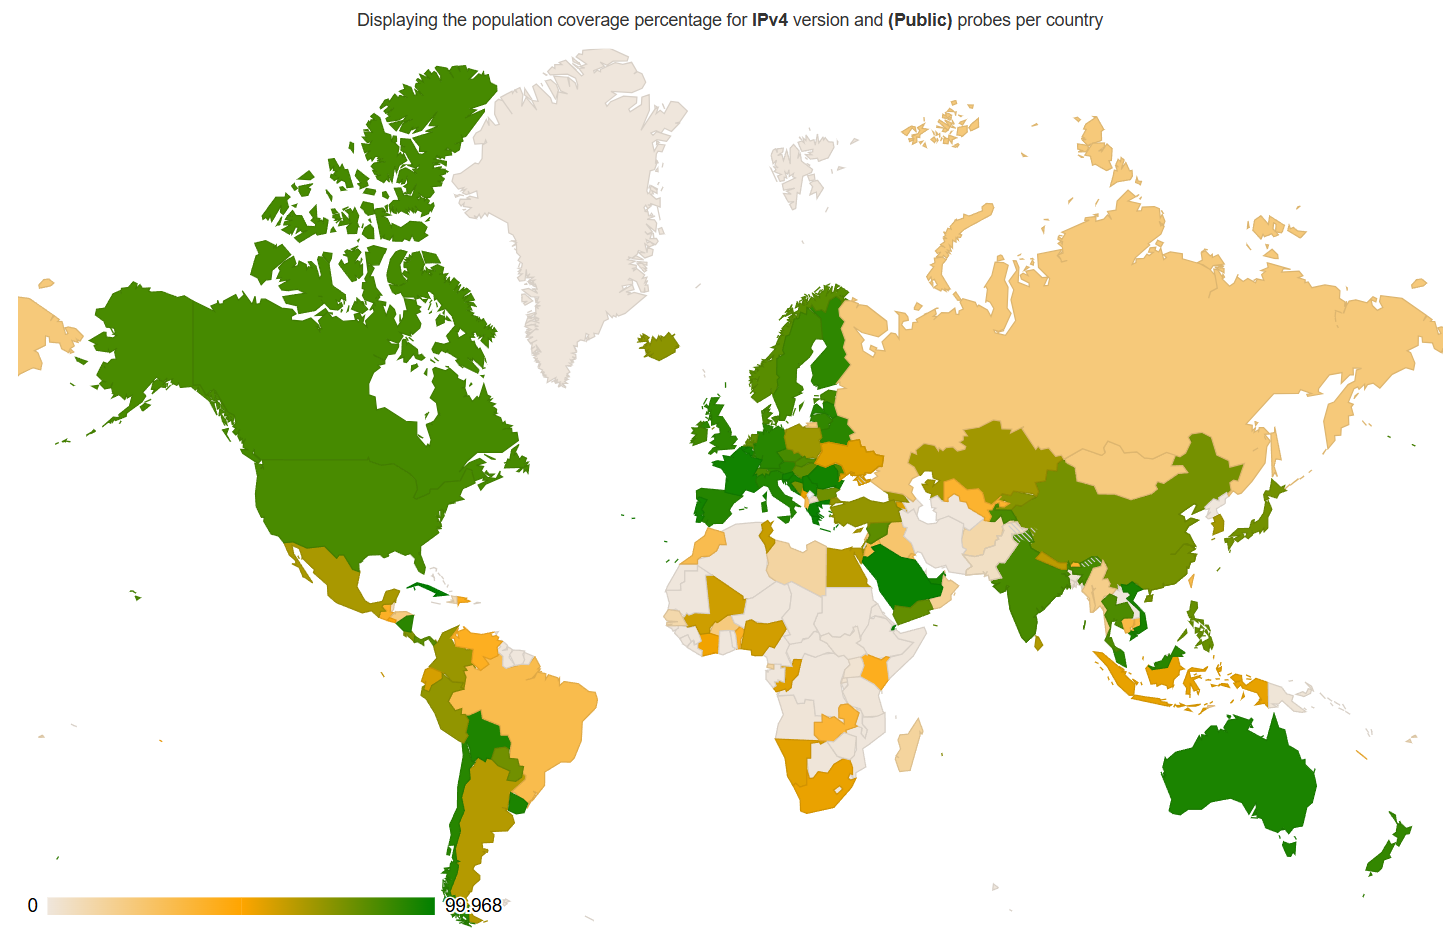
\includegraphics[width=0.90\linewidth]{figures/fig3b_ripe_atlas_distribution.png}
  \caption{Number of connected RIPE Atlas probes and anchors per country in March 30, 2026. Source: RIPE Atlas}
  \label{fig:ripe_atlas_distribution}
\end{figure}

Jones~\cite{Jones2016} detect in-path transparent \ac{DNS} proxies in ten \ac{ISP}s: a Kenyan \ac{ISP}'s proxy answers root \ac{DNS} queries 23× faster than the actual B-root \ac{RTT} (14 ms vs. 318 ms). Nosyk~\cite{Nosyk2025} find that 69\% of Chinese probes fail to resolve Meta domains — geographic filtering, not measurement failure. Both issues are detectable — \ac{RTT} sanity checks catch proxied probes; cross-domain cross-temporal comparison distinguishes censorship from hardware failure. A third data quality concern comes from Boswell and Perkins~\cite{Boswell2024}: 3,092 internal domain names are actively queried by RIPE Atlas probes, 34.5\% of which risk name collision if their \ac{TLD} is ever globally delegated. Probe resolution behaviour must be validated before including any probe in a corpus measurement.

\section{Anycast Routing in DNS}
\label{sec:2.4}

\ac{IP} anycast is the dominant routing architecture for \ac{DNS} root servers, \ac{TLD} servers, and major public resolvers (Google 8.8.8.8, Cloudflare 1.1.1.1). Probes at different geographic locations may contact physically different servers behind the same anycast \ac{IP}; the responses may differ in latency and, when servers are misconfigured or \ac{BGP} routing is suboptimal, in content. Three aspects of anycast matter for this thesis: instance identification (which server actually answered?), \ac{BGP} attraction basins (what topology shapes probe-to-instance routing?), and \ac{IPv4}/\ac{IPv6} divergence (do the two stacks route to the same instance?).

Anycast hides which server actually answered. Two mechanisms expose it. \ac{NSID}~\cite{RFC5001} asks the server to embed a string in the response: \texttt{dns.th2.nic.fr} tells you the Paris instance of \texttt{d.nic.fr} answered. The CHAOS-class \texttt{id.server} query~\cite{RFC4892} returns an airport code — \texttt{ams}, \texttt{fra}, and so on. CHAOS replies are not cached, so the answer always comes from the live \ac{BGP}-routed instance~\cite{Finnegan2018}. Without one of these two mechanisms, two probes returning the same \ac{IP} are ambiguous: same physical server, or two different machines sitting behind the same anycast address?

Once instance identity is established, the question becomes: what governs which probes reach which instance? Bortzmeyer~\cite{Bortzmeyer2013} demonstrates for \texttt{d.nic.fr} that anycast routing is governed by \ac{BGP} peering topology rather than physical distance. While one might expect North American queries to be routed to the geographically closest node, 55\% are sent to Paris and 33\% to Frankfurt — network closeness in \ac{BGP} does not align with mileage. Finnegan~\cite{Finnegan2018} confirms this pattern for UncensoredDNS with 500 Atlas probes. For this thesis, the implication is concrete: geographically diverse probes do not automatically sample diverse anycast instances — a response difference between probes may be a \ac{BGP} routing artefact, not a \ac{CDN} policy.

\ac{IPv4}/\ac{IPv6} divergence is a related issue. The IPv4 and IPv6 \ac{BGP} routing tables are managed independently. An anycast prefix announced over both stacks can resolve to different physical servers depending on which stack carries the query. Bortzmeyer measured this for \texttt{d.nic.fr}~\cite{Bortzmeyer2013}: Frankfurt answered 36\% of IPv6 queries, but only 17\% of IPv4. Second place in one stack, not in the other. A measurement that mixes IPv4 and IPv6 queries cannot treat them as interchangeable. Koch adds a related issue~\cite{Koch2021}: anycast inflation, where queries land on a suboptimal replica, affects over 95\% of users for at least one root-server letter. Root records cache for six days — tolerable. CDN A records with 60-second TTLs — not tolerable.

\section{CDN Routing and EDNS Client Subnet}
\label{sec:2.5}

\ac{CDN}s use \ac{DNS} as the primary mechanism to direct each client to a geographically appropriate server replica. The \ac{CDN}'s authoritative server returns a different \ac{A}/\ac{AAAA} record depending on the inferred location of the querying resolver. Li~\cite{Li2025}, studying Twitch, find continent-level \ac{DNS} routing granularity: distinct \ac{IP} groups are returned to probes in Europe, North America, and Asia-Pacific, creating sharp geographic boundaries detectable by distributed active measurement.

Geographic \ac{CDN} routing works by inspecting the resolver's \ac{IP} address, not the user's. When resolver and user are co-located, the inference is valid. When they are not, it fails --- a Namur user querying Google 8.8.8.8 gets California-region \ac{CDN} routing, not European. Hours quantified the penalty from passive \ac{ISP} traces~\cite{Hours2016}: clients behind Google's resolver reached Akamai servers 20~ms farther away on average, losing 14\% of throughput to tighter TCP congestion windows. Wang tracked public \ac{DNS} adoption growing at 27\% per year~\cite{Wang2018}; by their measurement window, routing mismatches had already reached 113\% of optimal server distance. The problem was growing, not shrinking.

\ac{ECS}~\cite{RFC7871} patches the mismatch by embedding the client's /24 prefix in the query, letting the \ac{CDN} route on the client's actual location rather than the resolver's. The catch is privacy — the client subnet is visible to the authoritative server and any on-path device, which is why RFC~7871 makes \ac{ECS} opt-in and recommends disabling it by default. Bortzmeyer~\cite{Bortzmeyer_tutorial} checked: most RIPE Atlas probes run resolvers that strip \ac{ECS} headers, so responses remain resolver-\ac{IP}-determined unless the measurement explicitly sends SOURCE PREFIX-LENGTH = 0. Figure~\ref{fig:ecs_schema} shows all three cases.

\begin{figure}[tp]
  \centering
  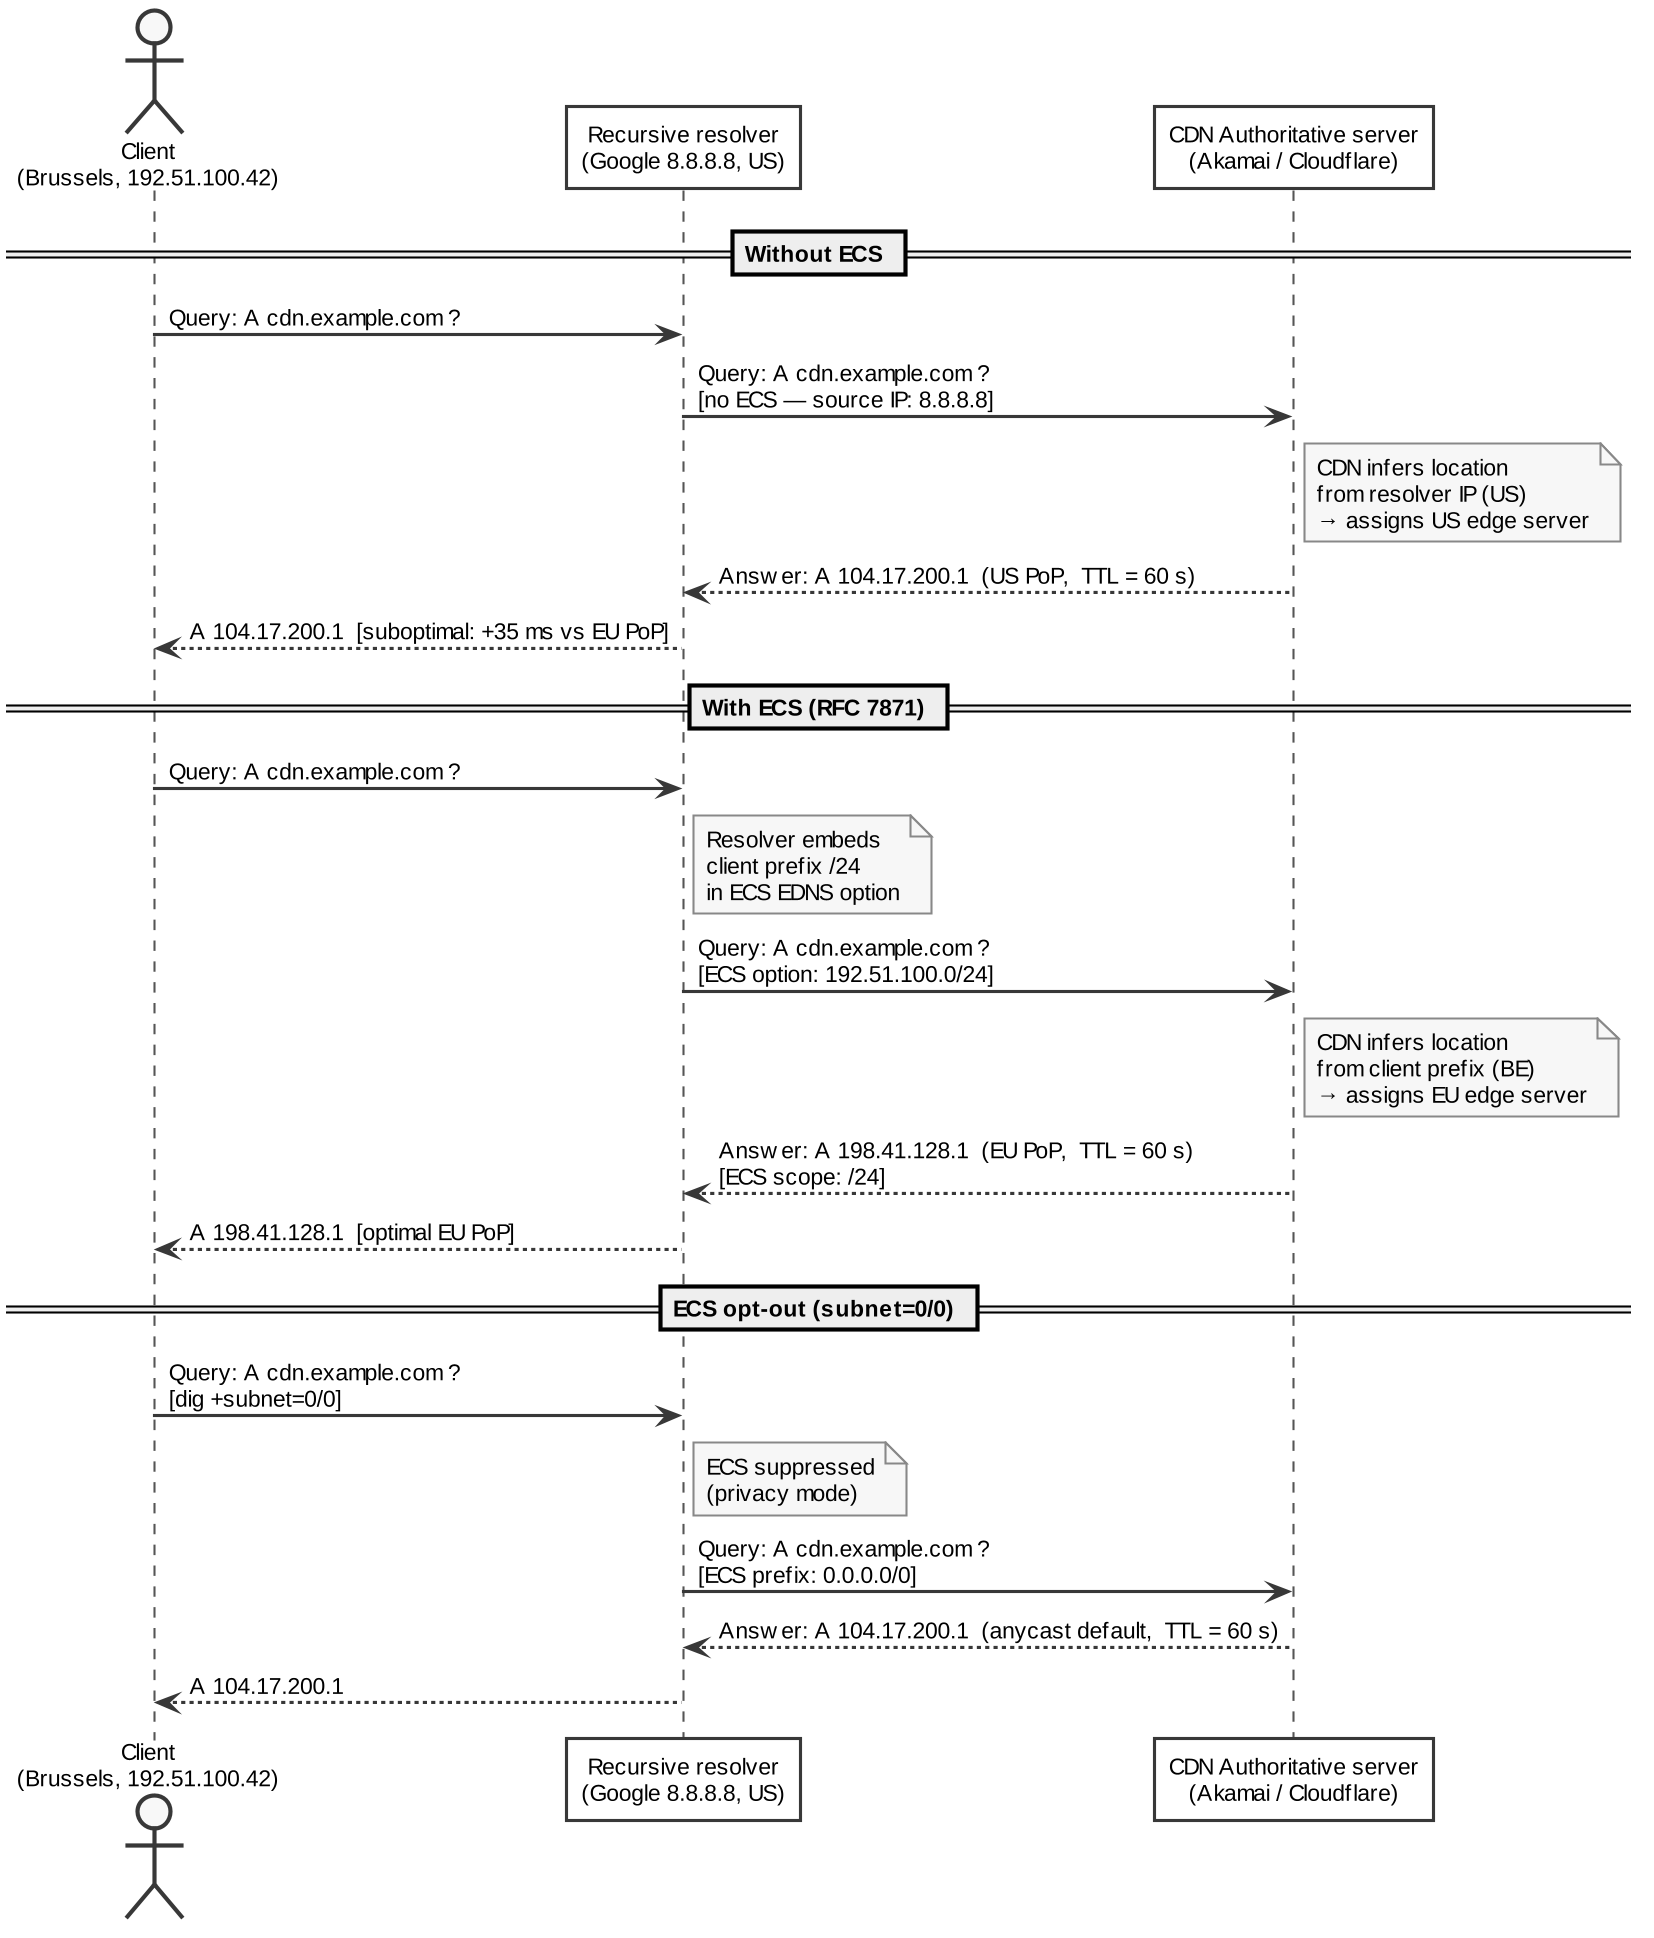
\includegraphics[width=0.90\linewidth]{figures/fig4_ecs_schema.png}
  \caption{Effect of \ac{ECS}~\cite{RFC7871} on \ac{CDN} geographic routing. \textit{Without \ac{ECS}}, the \ac{CDN} authoritative server infers client location from the recursive resolver's \ac{IP} (8.8.8.8, US), assigning a suboptimal US edge server to a Belgian client. \textit{With \ac{ECS}}, the resolver embeds the client's /24 prefix; the \ac{CDN} selects the geographically appropriate EU \ac{PoP}. \textit{\ac{ECS} opt-out} (\texttt{subnet=0/0}) suppresses the prefix entirely, reverting to resolver-\ac{IP}-based routing.}
  \label{fig:ecs_schema}
\end{figure}

Xu~\cite{Xu2023} show that \ac{DNS} infrastructure is more concentrated than it appears: over 90\% of forwarding resolvers are backed by fewer than 5\% of indirect recursive resolvers, and just 10 providers serve 48.5\% of all g\ac{TLD} domain names. Two probes on opposite continents sharing the same upstream recursive resolver return indistinguishable answers regardless of their physical location. Geographic probe diversity becomes illusory.

Two measurement modes address this differently. \textit{Using the probe's default resolver} captures the full recursive resolution chain --- \ac{ISP} cache, \ac{ECS} forwarding behaviour, all of it --- which is what real end-users actually experience. The resolver diversity problem is real, but it is also the phenomenon that Q4 measures. \textit{Querying the authoritative server directly} --- clearing the \ac{RD} bit and sending to the authoritative \ac{IP} --- bypasses the recursive layer entirely. The query arrives at the authoritative server from the probe's own \ac{IP}; the \ac{CDN}'s geographic routing policy applies to the probe's location, not a shared resolver in Virginia. RIPE Atlas supports both modes natively.

Q1--Q3 use the direct approach to characterise the authoritative layer's geographic routing in isolation. Q4 uses the default resolver to measure exactly what the direct approach cannot: how much resolver choice changes the answer a user actually receives.

\section{Domain Ranking Lists}
\label{sec:2.6}

Reproducibility is the first constraint on corpus choice for \ac{DNS} measurement: a domain list that shifts daily cannot support longitudinal comparisons. Le Pochat~\cite{LePochat2019} evaluated four freely available ranking lists — Alexa, Cisco Umbrella, Majestic, and Quantcast — and found they agree on only 70,000 of a combined 2.82 million unique domains (24–33\% rank-biased overlap). Alexa's 2018 methodology change caused 50\% daily list turnover, making longitudinal studies unreliable; Amazon subsequently shut down the Alexa ranking service entirely on 1 May 2022, making it unavailable for any ongoing research. Cisco Umbrella contains 51\% non-web entries (EC2 hostnames, typos). Majestic contains 2,162 documented malicious domains. All four lists are trivially manipulable: a single \ac{HTTP} request from an Alexa browser extension user can lift a domain to rank 28,798. Table~\ref{tab:ranking_lists} compares the main properties.

\begin{table}[tp]
\centering
\small
\begin{tabularx}{\linewidth}{p{2.2cm} X X X X}
\toprule
\textbf{Property} & \textbf{Alexa} \newline \textit{(discontinued 2022)} & \textbf{Cisco Umbrella} & \textbf{Majestic} & \textbf{Tranco} \\
\midrule
Data source  & Browser extension & \ac{DNS} queries to OpenDNS & Web crawl backlinks & Multi-source aggregation \\
Daily change rate & $\approx$50\,\% (post-2018) & $\approx$10\,\% & $\approx$1\,\% & $\approx$0.6\,\% \\
Manipulation effort & 1 \ac{HTTP} request & 1 \ac{DNS} query injection & Few backlinks & 4$\times$ vs single-source \\
Non-domain entries & Low & $\approx$51\,\% & Low & Filtered \\
Malicious domains & Some & Some & 2\,162 documented & Filtered \\
Reproducibility   & Daily overwrite & Daily overwrite & Daily overwrite & Stable permalink \\
\bottomrule
\end{tabularx}
\caption{Comparison of domain ranking lists. Tranco is the only list designed for research reproducibility and manipulation resistance~\cite{LePochat2019}.}
\label{tab:ranking_lists}
\end{table}

Tranco~\cite{LePochat2019} combines four lists into a 30-day rolling ranking using the Borda count. To manipulate it, an adversary must game all four contributing lists simultaneously --- roughly four times the effort of attacking any single source --- which is why the daily churn rate sits at 0.6\%, an order of magnitude below Alexa's post-2018 figure. Each snapshot gets a permanent permalink; any researcher can pull the exact same 250 domains from the archive years later. For this thesis that matters concretely: all 50 measurement days draw from the same frozen snapshot, so any response change observed over time is a \ac{DNS} routing event, not a corpus turnover artefact.

\section{Synthesis and Research Positioning}
\label{sec:2.7}

The literature reviewed above leaves a clear gap. OpenINTEL holds eleven years of daily \ac{TLD}-wide \ac{DNS} records — one server in the Netherlands, zero geographic coverage. RIPE Atlas has global reach — but every \ac{DNS} study that used it targeted a single service or a single moment: Bortzmeyer~\cite{Bortzmeyer2013} on \texttt{d.nic.fr} alone; Finnegan~\cite{Finnegan2018} on one resolver at one point in time; Hours~\cite{Hours2016} on a handful of \ac{CDN} providers in a one-shot campaign; Koch~\cite{Koch2021} photographing root-server anycast at a single point in time. Nobody has asked the population-scale question across a corpus of popular domains: how widespread is geographic \ac{DNS} differentiation, which mechanisms drive it, and does the picture stay stable over weeks and months? Table~\ref{tab:gap_analysis} lays out the positioning.

\begin{table}[tp]
\centering
\small
\begin{tabularx}{\linewidth}{p{2.8cm} p{3.5cm} p{3.8cm} X}
\toprule
\textbf{Dimension} & \textbf{OpenINTEL-based studies}~\cite{vanRijswijk2016} & \textbf{Existing RIPE Atlas studies}~\cite{Bortzmeyer2013,Finnegan2018,Hours2016,Koch2021} & \textbf{This thesis} \\
\midrule
Domain coverage  & Full \ac{TLD} zone files & Experimenter-defined (per study) & Tranco Top-250 (stable, reproducible) \\
Geographic vantage    & Single point (Netherlands) & $\approx$12\,900 probes, 178 countries & Multi-continent stratification \\
Temporal depth & Daily since March 2015 & Single campaigns & 50-day repeated campaigns \\
Anycast tracking       & Not applicable & Case studies (d.nic.fr, UncensoredDNS) & Systematic across corpus \\
Resolver control   & Fixed central resolver & Local probe resolver (default) & Direct authoritative query \\
\bottomrule
\end{tabularx}
\caption{Positioning of this thesis relative to existing \ac{DNS} measurement infrastructure across five dimensions.
All three columns represent measurement studies; Each row identifies a gap that this work explicitly addresses.}
\label{tab:gap_analysis}
\end{table}

The table has three rows. Each row names something the existing literature does not answer.

\textit{Gap 1 --- Population-scale geographic characterisation.} Bortzmeyer~\cite{Bortzmeyer2013}, Finnegan~\cite{Finnegan2018}, Hours~\cite{Hours2016}, and Li~\cite{Li2025} each pick one service and run one campaign. The population-scale question stays unasked: what fraction of popular domains return different answers by probe origin? Which mechanism is responsible --- anycast topology, \ac{CDN} routing policy, or \ac{ECS}?

\textit{Gap 2 --- Resolver centralisation swallows probe diversity.} Xu~\cite{Xu2023} show that 90\% of forwarding resolvers pass through just 5\% of recursive resolvers. Two probes on opposite continents sharing the same upstream return identical answers regardless of their physical locations. None of the cited studies use direct authoritative queries as a fix.

\textit{Gap 3 --- Single-campaign studies cannot see routing change.} Koch~\cite{Koch2021} and Bortzmeyer~\cite{Bortzmeyer2013} both note that \ac{BGP} peering and anycast catchments shift as operators add \ac{PoPs}. They note this in studies that are themselves one-shot. Whether geographic \ac{DNS} differentiation is stable over weeks and months is not answerable from a snapshot --- theirs or anyone else's.

Chapter~\ref{ch:method} targets all three: Tranco Top-250 queried at authoritative servers from $\approx$200 geographically stratified RIPE Atlas probes, daily for 50 days, with \ac{NSID}-based anycast tracking, results in Parquet under \ac{FAIR} principles.
